\documentclass{article}
\usepackage[preprint]{neurips_2026}
\usepackage[utf8]{inputenc}
\usepackage[T1]{fontenc}
\usepackage{microtype}
\usepackage{amsmath,amssymb}
\usepackage{booktabs}
\usepackage{array}
\usepackage{multirow}
\usepackage{graphicx}
\usepackage{xcolor}
\usepackage{hyperref}
\usepackage{url}
\usepackage{enumitem}
\usepackage{tikz}
\usetikzlibrary{arrows.meta,positioning,fit}
\hypersetup{
  colorlinks=true,
  linkcolor=black,
  citecolor=black,
  urlcolor=blue,
  pdfauthor={Aura Yavary},
  pdftitle={TraceSurgery: Replay-Controlled Counterfactual Evaluation of Failure Causality in Computer-Use Agents},
  pdfsubject={Computer-use agents, causal evaluation, counterfactual replay, failure diagnosis},
  pdfkeywords={computer-use agents, agent evaluation, causal debugging, counterfactual replay, recovery}
}
\setlist[itemize]{leftmargin=*,nosep}

\title{TraceSurgery: Replay-Controlled Counterfactual Evaluation\\of Failure Causality in Computer-Use Agents}

\author{
  Aura Yavary \\
  University of California, Davis
}

\begin{document}
\maketitle

\begin{abstract}
Computer-use agents increasingly operate long, stateful workflows in browsers and desktop applications, yet a failed final state says little about what actually caused the failure or whether the trajectory was still recoverable. Existing work already provides realistic computer-use environments, failure taxonomies, critical-step localization, recovery benchmarks, and counterfactual repair. We study a narrower question: \emph{when a debugger claims that a particular step or mechanism caused a failure, does an executed intervention at that checkpoint actually change the outcome?} We introduce \textbf{TraceSurgery}, an evaluation framework that treats failed trajectories as branchable experiments. For each checkpoint, TraceSurgery first replays the unmodified suffix to establish replay fidelity; only replay-faithful checkpoints are eligible for causal interpretation. It then applies controlled action, world-state, internal-state, or continuation interventions and re-grades the resulting environment state. These branches define a \emph{counterfactual recovery surface} over intervention time and intervention family, enabling diagnosis-faithfulness tests, last-recoverable-checkpoint estimates, intervention-type decomposition, and recovery-cost accounting. The released implementation includes checkpoint provenance, evidence gates, task-level statistics, a reproducible deterministic case study, and an auditable claim ledger. In the executed local case study, both no-intervention controls reproduce the source failure, while the effective repair family changes across checkpoints: an action or suffix repair succeeds before state corruption, whereas a state repair succeeds only after corruption. We intentionally report no frontier-model performance; realistic multi-model experiments are required before making capability or state-of-the-art claims.
\end{abstract}

\section{Introduction}

Long-horizon computer use is an unusually demanding setting for agent reliability. A single task may span hundreds of actions, multiple applications, changing external state, delayed effects, partially observed constraints, and safety-sensitive operations. OSWorld introduced a reproducible desktop environment for open-ended computer tasks~\citep{xie2024osworld}; OSWorld 2.0 subsequently emphasized much longer workflows in which current frontier systems still lose constraints, miss changing information, skip verification, and struggle with hidden state~\citep{yuan2026osworld2}. WebArena and BrowserGym expose related challenges in realistic web environments and standardized evaluation infrastructure~\citep{zhou2023webarena,dechezelles2025browsergym}.

A binary success label is necessary but insufficient for understanding these failures. Consider two failed trajectories with identical final scores. In one, the agent takes a single wrong action but remains in a recoverable state; in the other, an early mistake corrupts the world state and makes later reasoning irrelevant. From the final label alone, these failures look identical. A post-hoc explanation may identify a plausible root cause, but plausibility is not the same as causal sufficiency.

Recent work has made substantial progress on failure diagnosis and recovery. AgentErrorBench and AgentDebug systematize agent failure taxonomies and debugging~\citep{zhu2025agentdebug}. AgentRx localizes critical failure steps from execution trajectories~\citep{barke2026agentrx}. CUADebug targets computer-use agents specifically, combining a CUA error taxonomy, human-annotated failures, root-cause analysis, and re-execution~\citep{zhang2026cuadebug}. GUI-RobustEval and RoTS evaluate policy-induced error recovery and synthesize recovery data~\citep{bu2026rots}. CausalFlow uses step-level intervention to derive counterfactual repairs~\citep{bonagiri2026causalflow}, while MRFR/GCJR studies inclusion-minimal repair families under counterfactual replay~\citep{li2026mrfr}. These works make it inappropriate to claim novelty for ``failure taxonomy,'' ``counterfactual repair,'' or ``recovery'' in isolation.

TraceSurgery therefore adopts a deliberately narrower contribution: \textbf{replay-controlled causal evaluation of failure mechanisms in computer-use trajectories}. The core methodological requirement is simple: before interpreting an intervention branch, replay the same checkpoint with the same suffix and verify that it reproduces the source outcome under a declared state-equivalence policy. If the control cannot reproduce the source, the intervention may still be operationally interesting, but it is not admissible as clean causal evidence.

This framing leads to four contributions:
\begin{itemize}
  \item \textbf{Counterfactual recovery surfaces.} We evaluate recoverability jointly over checkpoint time and intervention family rather than reporting a single recovery rate.
  \item \textbf{Replay-fidelity gating.} Causal summaries exclude checkpoints whose no-intervention controls fail to reproduce the source trajectory under the preregistered equivalence rule.
  \item \textbf{Mechanism-level intervention decomposition.} Action, world-state, internal-state, and continuation interventions test different causal hypotheses about where failure resides.
  \item \textbf{Auditable evidence discipline.} Branch provenance, a claim ledger, and evidence gates keep software-validation evidence separate from scientific model-performance evidence.
\end{itemize}

The current release validates the framework semantics and a deterministic case study. It does \emph{not} establish superiority over existing debuggers or recovery methods. A publishable empirical conclusion requires realistic checkpointable environments, matched baselines, repeated model trials, human calibration, and task-level uncertainty.

\section{Related work and novelty boundary}

\paragraph{Computer-use evaluation.}
OSWorld~\citep{xie2024osworld} and OSWorld 2.0~\citep{yuan2026osworld2} provide realistic desktop workflows with execution-based grading. WebArena~\citep{zhou2023webarena} focuses on realistic self-hosted web environments, and BrowserGym~\citep{dechezelles2025browsergym} unifies web-agent evaluation across benchmarks. These environments motivate TraceSurgery but solve a different problem: they primarily measure whether a task succeeds, whereas TraceSurgery asks what intervention would have changed the outcome and when recovery ceases to be possible.

\paragraph{Failure localization and debugging.}
AgentDebug~\citep{zhu2025agentdebug} and AgentRx~\citep{barke2026agentrx} formalize failure attribution in agent trajectories. CUADebug~\citep{zhang2026cuadebug} is especially close in domain: it localizes causal errors in computer-use trajectories and evaluates diagnosis-guided re-execution. TraceSurgery is complementary. Rather than scoring a diagnosis primarily against human labels or downstream re-execution, it asks whether a declared mechanism survives a controlled intervention test at a replay-faithful checkpoint.

\paragraph{Recovery and counterfactual repair.}
GUI-RobustEval/RoTS~\citep{bu2026rots} focuses on robustness to policy-induced errors and large-scale recovery-data synthesis. CausalFlow~\citep{bonagiri2026causalflow} applies step-level counterfactual intervention and minimal edits, while MRFR/GCJR~\citep{li2026mrfr} recovers minimal repair families in multi-agent traces. TraceSurgery does not claim minimal repair as new. Its focus is the \emph{geometry} of recoverability across time and intervention type, with replay fidelity serving as an explicit admissibility condition.

\paragraph{Environment validity.}
Counterfactual replay is only meaningful if the environment itself preserves task-relevant context. GUI-CC shows that plausible one-step GUI generation can still fail under repeated multi-step rollout~\citep{fu2026guicc}. This motivates separating environment-replay validity from agent-repair effect and treating failed controls as a reason to withhold causal interpretation.

\section{Problem formulation}

Let a failed computer-use trajectory be
\begin{equation}
\tau = (o_0,a_0,s_0,o_1,a_1,s_1,\ldots,o_T,a_T,s_T),
\end{equation}
where $o_t$ is the agent-visible observation, $a_t$ is the action, and $s_t$ is evaluator-only environment state. A task grader $G(s_T)\in\{0,1\}$ maps the final state to task success. We focus on a source trajectory with $G(s_T)=0$.

An intervention family $I$ at checkpoint $t$ creates a branch $\tau^{(t,I)}$ and final state $s_T^{(t,I)}$. The counterfactual outcome is
\begin{equation}
R(t,I)=G\!\left(s_T^{(t,I)}\right).
\end{equation}
The matrix $R$ over checkpoints and intervention families is the \textbf{counterfactual recovery surface}.

\subsection{Replay fidelity as an admissibility condition}
A branch can only support a clean causal interpretation if the checkpoint itself is reproducible. We therefore execute a no-intervention control from the same checkpoint using the recorded suffix. Let $E(\cdot,\cdot)$ be a preregistered task-relevant equivalence relation over final states. Checkpoint $t$ is admissible when
\begin{equation}
E\!\left(s_T^{(t,\varnothing)}, s_T\right)=1.
\end{equation}
For deterministic sandboxes, $E$ may be exact state equality or a stable state hash. For stochastic GUI systems, $E$ must be defined before examining intervention outcomes and should compare only task-relevant state. If the control fails, TraceSurgery stores the intervention result but excludes it from causal summaries.

\subsection{Causal effect and recovery surface summaries}
For a failed source outcome $Y_0=0$ and branch outcome $Y(t,I)$, the direct branch effect is
\begin{equation}
\Delta(t,I)=Y(t,I)-Y_0.
\end{equation}
Because multiple branches descend from the same source trajectory, branches are correlated and must not be treated as independent samples in statistical tests.

For a fixed intervention family $I$, we define the last recoverable checkpoint (LRC) as the latest admissible checkpoint with $R(t,I)=1$. A normalized recovery AUC summarizes the mean recovery indicator over admissible checkpoints. These summaries are descriptive unless task-level repeated trials support inferential analysis.

\section{TraceSurgery}

Figure~\ref{fig:architecture} shows the evaluation loop. A source failure is checkpointed. For each checkpoint, a control branch verifies replay fidelity; admissible checkpoints are then subjected to intervention families and re-graded. The resulting surface can score debugger claims, identify irreversibility boundaries, and distinguish whether recovery requires changing an action, repairing the world state, repairing internal state, or changing the future policy.

\begin{figure}[t]
\centering
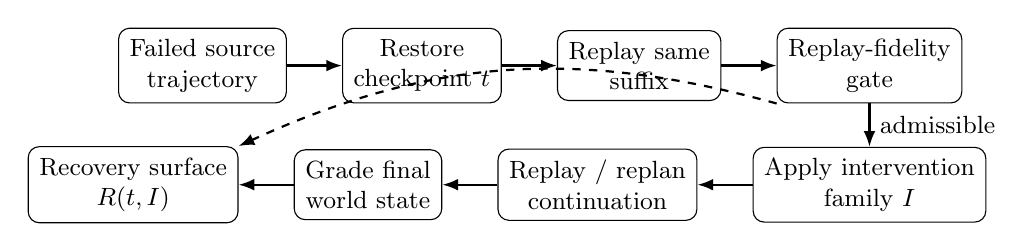
\begin{tikzpicture}[node distance=5.5mm and 7mm, every node/.style={font=\small}, box/.style={draw,rounded corners,align=center,minimum height=7mm,inner sep=4pt}, arr/.style={-{Latex[length=2mm]},thick}]
\node[box] (src) {Failed source\\trajectory};
\node[box,right=of src] (cp) {Restore\\checkpoint $t$};
\node[box,right=of cp] (ctrl) {Replay same\\suffix};
\node[box,right=of ctrl] (gate) {Replay-fidelity\\gate};
\node[box,below=of gate] (int) {Apply intervention\\family $I$};
\node[box,left=of int] (replay) {Replay / replan\\continuation};
\node[box,left=of replay] (grade) {Grade final\\world state};
\node[box,left=of grade] (surf) {Recovery surface\\$R(t,I)$};
\draw[arr] (src)--(cp);
\draw[arr] (cp)--(ctrl);
\draw[arr] (ctrl)--(gate);
\draw[arr] (gate)-- node[right]{admissible} (int);
\draw[arr] (int)--(replay);
\draw[arr] (replay)--(grade);
\draw[arr] (grade)--(surf);
\draw[arr,dashed] (gate.south west) to[bend right=20] (surf.north east);
\end{tikzpicture}
\caption{TraceSurgery converts a failed trajectory into controlled branch-and-replay experiments. The no-intervention branch is not a baseline afterthought; it is a gate that determines whether intervention branches at checkpoint $t$ are causally admissible.}
\label{fig:architecture}
\end{figure}

\subsection{Intervention families}
Table~\ref{tab:interventions} lists the intervention families and their intended causal questions. Importantly, evaluator-side surgery is not evidence that an agent can autonomously recover. Oracle interventions estimate causal structure and upper bounds; agent-realizable recovery requires a separate policy or debugger comparison.

\begin{table}[t]
\centering
\small
\begin{tabular}{p{0.20\linewidth}p{0.69\linewidth}}
\toprule
\textbf{Intervention} & \textbf{Question tested} \\
\midrule
No intervention & Does the same checkpoint and suffix reproduce the source outcome? \\
Action patch & Was the action at checkpoint $t$ causally sufficient under the fixed continuation? \\
Observation refresh & Was a stale or corrupted observation the bottleneck while world state remained fixed? \\
State patch & Was accumulated external-state corruption sufficient to explain the failure? \\
Belief/memory patch & Was exposed internal state inconsistent with the task-relevant world state? \\
Local replan & Can a bounded next-action correction recover without rollback? \\
Suffix replan & Is the current world state still salvageable under a better continuation policy? \\
Rollback + replan & How far must execution be rolled back before recoverability returns? \\
\bottomrule
\end{tabular}
\caption{Intervention families. Not all families are available for every agent architecture; unsupported interventions must be reported rather than silently approximated.}
\label{tab:interventions}
\end{table}

\subsection{Diagnosis faithfulness}
Suppose a debugger emits a structured claim $D=(t,I)$: checkpoint $t$ is the root cause and intervention family $I$ is the appropriate repair. We call the claim \textbf{intervention-faithful} only if (i) the checkpoint is replay-faithful and (ii) the declared repair has positive executed outcome effect. This criterion intentionally distinguishes a plausible explanation from a falsifiable causal claim.

For multiple candidate diagnoses, evaluation can report precision over intervention-faithful claims, rank correlation between predicted causal strength and measured $\Delta(t,I)$, and calibration of confidence against realized repair effect. Human labels remain useful, but they are no longer the only target: a diagnosis can agree with an annotator yet fail to alter the outcome under controlled intervention.

\subsection{Provenance and contamination boundaries}
Every branch stores source-trial identity, checkpoint index, intervention kind, checkpoint hash, continuation hash, final-state hash, grader outcome, control-fidelity status, and causal-admissibility status. Ground-truth state is never exposed to the policy during ordinary execution. The implementation separates environment perturbations from agent-attributed failure events so that injected faults do not become automatic evidence of agent error.

\section{Metrics and statistical protocol}

TraceSurgery distinguishes branch-level descriptors from task-level scientific inference.

\paragraph{Branch-level metrics.}
Replay Fidelity measures the fraction of tested checkpoints that reproduce the source outcome and relevant final state. Recovery AUC summarizes recovery across admissible checkpoints for a fixed intervention family. LRC estimates the last point at which that intervention remains sufficient. Recovery cost includes added actions, latency, tokens, monetary cost, and safety side effects.

\paragraph{Task-level inference.}
If each task produces multiple branches and repeated stochastic rollouts, uncertainty must be clustered at the task or source-trajectory level. The released analysis code implements task-cluster bootstrap confidence intervals and paired task-level comparisons. Branches from one source trajectory are never counted as independent experimental units.

\paragraph{Matched comparisons.}
A paper-scale study should compare at least: (i) trace-only root-cause localization, (ii) diagnosis-guided re-execution, (iii) verifier-guided retry/replan, (iv) recovery-specialized policies, and (v) oracle intervention upper bounds. The key comparison is not whether TraceSurgery itself ``recovers more,'' because TraceSurgery is an evaluator. The question is whether diagnostic methods identify intervention points and repair mechanisms that produce measured causal effects.

\section{Executed deterministic case study}
\label{sec:case}

The current release contains a small deterministic case study whose role is to validate semantics, not to estimate model capability. A spreadsheet task requires writing a summary value of $42$ from inputs $[10,12,20]$. The source trajectory writes $41$ and then terminates. We checkpoint immediately before the write ($t=0$) and immediately after the corrupted state has been written ($t=1$), then execute four branch families at each checkpoint.

\begin{table}[t]
\centering
\small
\begin{tabular}{lccp{0.36\linewidth}}
\toprule
\textbf{Intervention} & $t=0$ & $t=1$ & \textbf{Interpretation} \\
\midrule
No intervention & Fail & Fail & Both controls reproduce the source failure. \\
Action patch & \textbf{Success} & Fail & Repair works before corruption, not after it. \\
State patch & Fail & \textbf{Success} & Before corruption the bad action re-corrupts state; after corruption state restoration is sufficient. \\
Suffix replan & \textbf{Success} & Fail & A better continuation helps only while the world state is still clean. \\
\bottomrule
\end{tabular}
\caption{Executed local case study. This is a deterministic semantic validation with two checkpoints, not a benchmark result and not evidence about frontier models.}
\label{tab:case}
\end{table}

Both no-intervention controls are replay-faithful. Three intervention branches change the final outcome. The important observation is not ``three successes''; it is that the effective repair mechanism changes with time. At $t=0$, changing the action or suffix is sufficient, whereas a state patch alone fails because the recorded bad action immediately reintroduces the corruption. At $t=1$, the incorrect value has already entered world state; changing the terminal action cannot fix it, and replaying the recorded suffix cannot undo it. A state patch now becomes the sufficient repair.

This example illustrates the motivation for recovery surfaces: a single label such as ``planning error'' or ``state error'' is temporally incomplete. The causal locus of recoverability can migrate as the consequences of an earlier decision become embedded in external state.

\subsection{Evidence layer}
The repository records the case study as raw branch JSON and derives the published table from those records. A claim ledger maps each public local claim to a raw evidence path and a verification rule. A standalone verifier recomputes replay-control counts, outcome-changing branch counts, checkpoint-specific repair patterns, and the published table. This machinery does not make the evidence more scientifically general; it makes the limited evidence auditable and harder to accidentally overstate.

\section{Paper-scale evaluation plan}

The central empirical hypothesis is that agents with similar task-success rates can have different \emph{failure geometry}: different distributions of repairable checkpoints, different intervention families that restore success, and different rates at which failures become irreversible.

A realistic study should use checkpointable browser/desktop environments and preserve the original task graders. Candidate environments include OSWorld/OSWorld 2.0 for desktop workflows and BrowserGym-hosted web benchmarks for browser tasks~\citep{xie2024osworld,yuan2026osworld2,dechezelles2025browsergym}. For each agent and task, failed source rollouts are replayed under matched seeds or controlled environment snapshots when possible.

We preregister the following research questions:
\begin{enumerate}[leftmargin=*]
  \item How often do trace-localized root causes correspond to interventions with positive executed outcome effect?
  \item What fraction of recoverable failures are primarily action-local, world-state-local, internal-state-local, or continuation-policy-local?
  \item How quickly does recoverability decay as intervention is delayed?
  \item Do similarly successful models exhibit different recovery surfaces and irreversibility boundaries?
  \item Which failure mechanisms become irreversible earliest?
  \item Does disagreement between agent belief and evaluator state predict which repair family is effective?
  \item How many apparent intervention effects disappear when replay-unfaithful checkpoints are excluded?
\end{enumerate}

\paragraph{Experimental unit and repetition.}
The source task/trajectory is the experimental unit. Multiple branches from one source remain correlated. Stochastic agents require repeated source rollouts and repeated branch rollouts with preregistered seeds or sampling controls. Confidence intervals should be task-clustered; paired methods should be used for comparisons on the same tasks.

\paragraph{Human calibration.}
Human annotators can label root-cause step, failure family, and candidate repair mechanism on a stratified subset. Agreement should be reported for both category and temporal localization. Human labels should not be treated as unquestioned causal ground truth; disagreement between human attribution and intervention effect is itself an informative outcome.

\paragraph{Cost and safety.}
Recovery quality must not be separated from cost or risk. A method that recovers by repeatedly restarting an application, issuing many expensive model calls, or attempting unsafe actions may be operationally inferior despite higher completion. We therefore report action overhead, model-call/token overhead, wall-clock latency, monetary cost when available, and safety violations separately from task success.

\section{Validity threats, limitations, and safety}

\paragraph{No frontier-model evidence in this release.}
The released deterministic case study validates framework semantics only. It cannot support claims about model ranking, typical failure distributions, or state-of-the-art recovery. The 500-task procedural suite in the repository is a software-validation suite, not a scientific benchmark dataset.

\paragraph{Replay assumptions.}
Causal inference depends on the quality of checkpoint restoration and state equivalence. In stochastic or partially external environments, exact replay may be impossible. The appropriate response is not to relax the gate after seeing results, but to preregister a task-relevant equivalence relation and report the fraction of checkpoints that remain admissible.

\paragraph{Intervention validity.}
Oracle action or state patches may use privileged evaluator information. They estimate causal sufficiency or upper bounds, not agent-realizable recovery. Every paper-scale experiment must clearly separate oracle surgery from policies that operate only on agent-visible information.

\paragraph{Intervention incompleteness.}
A failed repair does not prove the hypothesized mechanism is irrelevant if the intervention itself is misspecified. Conversely, a successful intervention can mask multiple interacting causes. Minimum repair-family analysis can reduce but not eliminate this ambiguity.

\paragraph{Environment validity.}
World-model or simulator-based replay can introduce its own failure modes. GUI-CC demonstrates that next-screen plausibility does not guarantee multi-step contextual consistency~\citep{fu2026guicc}. Realistic environment adapters therefore require their own transition and reset audits.

\paragraph{Safety.}
State rollback and automated replay must be isolated from irreversible real-world side effects. Destructive actions, purchases, external communication, account changes, and sensitive-data operations require sandboxing, permission boundaries, and explicit safety graders. TraceSurgery is designed as an evaluation tool, not a license to replay risky actions in production systems.

\section{Research engineering and reproducibility}

The implementation is provider-neutral and contains: (i) exact pre- and post-action observations, (ii) evaluator-only snapshots, (iii) perturbation events separated from agent failure attribution, (iv) checkpoint and continuation provenance hashes, (v) replay-fidelity gates, (vi) task-clustered statistical analysis, (vii) a concurrency-safe resumable experiment ledger, and (viii) an evidence gate that rejects local validation and synthetic demos from scientific performance summaries.

The external-study ledger expands a frozen study specification into task/model/environment/seed/repetition cells with deterministic run identifiers. A scientific-evidence record must identify the model revision, benchmark version, grader revision, and run-manifest provenance. When a manifest path is available, its SHA-256 is recomputed from disk before the record is eligible for scientific reporting. Reporting scripts fail closed rather than emitting publication tables from invalid evidence.

The repository also contains an evidence layer with experiment journal, failed investigations, decision log, real local eval tables, qualitative cases, raw branch artifacts, and a claim ledger. This process documentation is intentionally distinct from scientific experiments: engineering failures and deterministic semantic checks are not presented as model-evaluation trials.

\section{Discussion}

TraceSurgery changes the unit of analysis from ``which step looks wrong?'' to ``which intervention, applied when, changes the outcome under a reproducible replay substrate?'' This shift creates several opportunities.

First, failure explanations become falsifiable. A debugger that confidently identifies a critical step can be evaluated by intervening exactly there. Second, recoverability becomes a trajectory property rather than a single endpoint metric. Two agents can have identical task success yet differ in how late their failures remain salvageable. Third, the framework provides a bridge between evaluation and training: intervention-faithful repairs can define higher-quality supervision than unverified self-critiques, while replay-unfaithful regions identify environment or harness weaknesses rather than agent errors.

The strongest future result would not be a larger local demo. It would be a multi-model study showing that recovery surfaces reveal stable, decision-relevant differences that ordinary task success and trace-only diagnosis miss. The framework is constructed to make such a claim testable, while the current preprint keeps that claim explicitly unmade.

\section{Conclusion}

Reliable computer-use agents require more than successful final states and plausible post-hoc explanations. TraceSurgery operationalizes a stricter criterion for causal debugging: establish replay fidelity, intervene on a declared mechanism, execute the branch, and grade the resulting world state. The resulting recovery surface separates when a trajectory is salvageable from how it must be repaired. The current release provides an executable framework, provenance and evidence gates, and a deterministic case study in which the sufficient repair mechanism changes across checkpoints. The next scientific milestone is a realistic, repeated, multi-model evaluation with matched baselines and task-level uncertainty.

\bibliographystyle{plainnat}
\bibliography{references}

\appendix
\section{Reproducibility notes for the released case study}
The deterministic local demonstration is stored as a versioned JSON artifact in the project repository. The source task writes an incorrect spreadsheet summary and terminates. Reproduction consists of executing the source run, restoring each checkpoint, replaying the no-intervention suffix, and then executing the declared intervention branches. The evidence verifier recomputes the published branch counts and checkpoint-specific success pattern directly from raw branch records. The local case is intentionally small because its purpose is semantic regression testing, not statistical estimation.

\section{Recommended evidence hierarchy}
We recommend labeling results with one of three evidence scopes:
\begin{enumerate}
  \item \textbf{Software validation}: deterministic tests of framework semantics and invariants.
  \item \textbf{Controlled evaluation}: repeated experiments in realistic checkpointable environments with matched baselines and task-level uncertainty.
  \item \textbf{Deployment evidence}: observations from real operational settings with appropriate safety, privacy, and permission controls.
\end{enumerate}
Claims should not be promoted from one layer to the next solely because the same code path is used.

\section{NeurIPS-style transparency checklist for this preprint}
This arXiv preprint follows the NeurIPS 2026 preprint layout. The official conference checklist is required for an actual NeurIPS submission; the source package includes a style-source note explaining how to replace the local compatibility style with the official 2026 author-kit file before submission.

\begin{itemize}
  \item \textbf{Claims:} Yes. The abstract and introduction distinguish implemented evidence from planned external experiments.
  \item \textbf{Limitations:} Yes. Section 8 discusses replay assumptions, intervention validity, environment validity, lack of frontier-model evidence, and safety.
  \item \textbf{Theory assumptions/proofs:} N/A. The paper introduces definitions and evaluation methodology, not formal theorems.
  \item \textbf{Reproducibility:} Yes for the reported deterministic case study; external experiments are explicitly not reported.
  \item \textbf{Statistical significance:} N/A for the deterministic two-checkpoint case study; task-clustered inference is specified for future stochastic evaluations.
  \item \textbf{Compute:} Minimal for the released local validation. No frontier-model compute is claimed in this preprint.
  \item \textbf{Ethics and safety:} Discussed in Section 8, including isolation of irreversible actions and evaluator-state leakage boundaries.
\end{itemize}

\end{document}
